\documentclass[11pt]{article}

% Packages
\usepackage{amsmath}
\usepackage{graphicx}
\usepackage{amssymb}
\usepackage{longtable}
\usepackage[spanish]{babel}
\usepackage[utf8]{inputenc}
\usepackage[T1]{fontenc}
\usepackage{float}


\author{Brian Ameht Inclán Quesada C-411\\ Davier Sánchez Bello C-412\\ Eric López Tornas C-411}
\title{Proyecto Final de IA y Simulación \\ Juego de Supervivencia}
\date{}

% Document
\begin{document}

\maketitle
\newpage

\tableofcontents
\newpage

\section{Introducción}
Sugarscapes, expuesto extensamente en el libro "Growing Artificial Societies", publicado en 1996 bajo la autoria de Joshua Epstein y Robert Axtell es un modelo de simulacion clasico, que a traves de una simulacion bastante simple, con agentes de un comportamiento muy sencillo y pocos rasgos a modelar, logra simular con resultados muy realistas los comportamientos de las sociedades humanas en cuanto a distribucion de la riqueza, transmision cultural, reproduccion, combates, entre otros.
En SugarScapes, los agentes carecen de una verdadera IA detras de si, y son mas bien homogeneos a pesar de sus diferentes rasgos, debido a que todos actuan de manera similar en la mayor parte de las simulaciones inspiradas en SugarScapes.
Nosotros, quisimos explorar el tema de la violencia y la formacion de agrupaciones (bandas de gangster y demas) en la socieda, a traves de nuestra propia version de SugarScapes, pero cargando a los agentes de un comportamiento basado en IA. Queremos estudiar cuanto influyen el rango de vision, de movimiento, la riqueza heredada por un agente, su nivel de consumo, asi como la zona en que nacion en su supervivencia en un ambiente donde la reparticion de los recursos naturales que aparecen distribuidos de manera desigual esta signada por la ley del mas fuerte, por la violencia. Asi, algunos agentes eligiran asociarse a otros, bajo ciertas reglas de asociacion, mientras otro eligiran huir de los conflictos todo el tiempo y otros provocarlo. Cual de estas estrategias es mejor, es mejor la misma para cada tipo de agente en cuando a su capacidad de vision, movimiento y herencia, o para cada nivel de capacidad hay una estrategia que mas probablemente le asegure la supervivencia. Estas y otras preguntas que nos plantearemos son facilmente extrapolables, al igual que nuestra simulacion, a situaciones de la vida real, donde los individuos deben agruparse para tener mas fuerza y/o ejercerla sobre los demas, para sobrevivir, o inlcuso alcanzar mas poder.

\section{Modelo}
\subsection{Resumen del modelo}
Emparentado a Sugarscapes, nuestro modelo consiste en una grilla bidimensional, donde conviven diferentes tipos de agentes. Cada agente ocupa una casilla de la grilla, y cada casilla puede soportar una cantidad maxima de azucar, que varia para cada una. Todos los turnos las casillas que no han alcanzado su maximo potencial de azucar, incrementan en 1, aunq este parametro es ajustable, la cantidad de azucar que contienen. Cada vez que los agentes visitan una casilla, recogen todo el azucar presente en esta, e incrementan sus reservas en la cantidad de azucar recogida. Deben, todos los turnos, satisfacer su necesidad diaria de azucar, consumiendo sus propias reservas. Si en algun momento sus reservas caen de 0, mueren.
Los agentes podran interactuar entre si atacandose o haciendo asociaciones. Una asociacion es un pacto entre dos o mas agentes donde cada uno acuerda ceder un determinado por ciento de sus ganancias a la asociacion y luego a cada cual le corresponde una porcion de las ganancias totales de la asociacion. Pudieran ademas implementarse otras formas de relaciones sociales como las extorsiones.
Los agentes tendran diferentes rangos y formas de movimientos, de vision y de ataques, asi como naceran con diferentes necesidades de consumo y reservas.
\subsection{Ventajas}
La principal ventaja de este modelo de simulacion es que incluso tras introducir IA a los agentes y complejizar sus relaciones, la simulacion sigue siendo lo suficientemente simple como para incorporar un volumen considerable de agentes, de diferentes tipos, y correr un volumen suficiente de simulaciones como para llegar a conclusiones. Otra ventaja de este modelo es que, estando basado en la experiencia previa del Sugarscapes, sabemos y podemos comprobabr que emula muy bien los fenomenos ocurridos en la tan compleja sociedad humana, partiendo de una simulacion muy sencilla
\subsection{Desventajas}
La principal desventaja que encontramos en este modelo para estudiar las agrupaciones de violencia en las sociedades humanas es que no toma en cuenta la compatibilidad de caracter entre los agentes, o sea, todos los agentes pueden tener el mismo tipo de relaciones con todos los demas agentes. En la vida real, el caracter de algunas personas sles hace mas dificil e incluso imposible mantener algun tipo de relacion con otras personas, mientras que facilita el acercamiento entre otras. El modelo descrito realmente no toma en cuenta esta arista tan importante del factor humano.
\subsection{Posibles mejoras}
Respecto a la desventaja presentada anteriormente, se pudieran evaluar para incrementar en cuanto a realismo la simulacion, ciertas soluciones propuestas precisamente en el libro Growing Artificial Societies. En tal libro, se logra modelar caracteristicas culturales de los individuos como cadenas de bits donde ciertas propiedades de la cadena, ya fuera la posicion de los bits encendidos y apagados o la cantidad total de tales bits, sirven para agrupar a los agentes en diferentes categorizaciones, y sirven como su diferenciador cultural. Muy bien podriamos emplear esta variante para simular el caracter de los agentes y determinar cuales tienen relaciones mas fluidas con otros, lo cual pudiera ser un factor para retrasar sus comunicaciones, o que influya en sus tomas de decisiones.
Otra mejora que se pudiera hacer a la simulacion, y que parece obvia dado el tema escogido, es la introduccion de relaciones familiares entre los agentes, de manera que, al avanzar la simulacion, los clanes terminarian nucleando a una o unas pocas familias cada uno, y las relaciones familiares se convirtieran en un medio de poder, tal y como sucede en las agrupaciones mafiosas y las bandas violentas que intentamos emular.
Hablo aqui acerca d lo q nos falto hacer?

\section{Implementación}
\subsection{Modelo de la simulación}
La simulacion fue implementada de la manera mas escalable posible. Por tal motivo tenemos una interfaz ISimulation, que abstrae los metodos relativos a una simulacion que pueden ser modificados de una simulacion a otra, digase la forma de resolver los ataques o las propuestas de asociaciones. Comencemos hablando entonces de esta interfaz ISimulation y sus metodos no abstractos.
La simulacion es episodica, y simulamos cada episodio usando el metodo step. Cada episodio es una ejecucion de step. Fijamos la forma en que ocurre cada episodio, y es de la siguiente manera:
-Primeramente actualizamos a cada agente acerca de lo que puede ver, con la invocacion del metodo __actualize_agents_vision__
-Luego recogemos las propuestas de asociacion que cada agente desea realizar, usando el metodo __get_association_proposals__; asi como los ataques que cada agente desea realizar, usando el metodo __get_attacks__.
-Posteriormente son ejecutadas las propuestas de asociacion y los ataques en ese orden con los metodos declarados abstractos que fueron mencionados anteriormente
-Luego se recogen las intenciones de movimiento de cada agente, con __get_moves__, y se ejecutan con __execute_moves__.
-Luego cada agente incrementa sus reservas acorde a la cantidad cosechada en la casilla en que se encuentra y mas tarde consume la cantidad que debe consumir. Los agentes cuyas reservas alcanzan numeros negativos, senhal de que no les alcanzo para satisfacer sus necesidades son retirados de la simulacion.
-Finalmente, cada casilla que no haya alcanzado la cantidad de azucar acumulada maxima, incrementa en 1 su cantidad de recursos
Ahora vayamos a fondo y veamos de que manera funciona cada uno de estos metodos, asi como la descripcion de los tipos usados en la simulacion.
Toda simulacion cuenta con un Map, y con un diccionario llamado agents que para cada id de agente le hace corresponder un Agent_Handler.
El mapa de una simulacion almacena tres tipos de informacion, la informacion relativa a la presencia de agentes y objetos en las diferentes posiciones, la informacion relativa a la cantidad de azucar en cada posicion y la informacion relativa a las acciones que han sido ejecutadas desde una determinada posicion en el turno anterior. Dado que asumimos que en toda casilla puede haber solo un agente o solo un objeto, y todo objeto o agente de la simulacion tiene un id unico, entonces dada la biyeccion entre las posiciones del tablero y aquello que almacenan, manejamos las posiciones de agentes y objetos usando un bidict, estructura de python para tuplas donde se puede hacer un lookup en O(1) tanto por llave como por valor. La informacion de la cantidad de azucar en cada casilla, la cantidad maxima de azucar en cada casilla y las acciones ocurridas en el ultimo turno, son manejadas usando diccionarios comunes de python.
El mapa presenta metodos para insertar o mover objetos o agentes, insertar acciones, eliminar agentes o objetos en una posicion especifica o con un id especifico, asi como averiguar la posicion de un agente u objeto con un id especifico, o averiguar el contenido de una casilla en especifico. Ademas el mapa tiene metodos para aumentar en 1 la cantidad de azucar que tiene cada casilla no llena y para que cada agente coseche la cantidad de azucar que le corresponde debido a la casilla en que se encuentra.
Las acciones son almacenadas en el mapa como una lista por cada posicion con las acciones tomadas desde esa posicion en el turno anterior. Tales acciones son representadas por instancias de la clase Action o de la clase Action_Info, o alguno de los tipos que heredan de ellos. Ambas jerarquias de tipo se usan para guardar para su transformacion informacion relatva a los eventos de la simulacion, y se usan, al menos en el caso de su presencia dentro de Map, para informar al agente acerca de lo que ha ocurrido a su alrededor.
Las simulaciones cuentan ademas, como habiamos mencionado anteriormente con un diccionario que para cada id de agente le hace corresponder un Agent_Handler. Agent_Handler es la clase encargada de manejar toda la informacion relativa a un agente de la simulacion, establecer comunicacion con el, informandole de todo aquello que puede ver, las acciones que lo afectan y ademas preguntandole que acciones desea realizar y verificando si tales acciones son validas. Dentro de la informacion que guarda Agent_Handler encontramos por ejemplo las asociaciones a que pertenece, quienes son sus aliados, su nivel de azucar, el porciento de sus ganacias que no ha comprometido aun con ninguna organizacion, su consumo dirario etc.
La capacidad de movimiento de un agente, su rango de vision y de ataque, estan dados por instancias de las interfaces IMovement, IVision, IAttack_Range y tanto el Agent_Handler como el propio agente son informados de sus capacidades, de manera que el Agent_Handler puede descartar cualquier accion del agente que no sea valida, asi como el agente esta en condiciones de deducir que acciones puede tomar.
Los agentes cumplen con la interfaz IAgent que plantea la API a traves de la cual los agentes se comunican. Esta API tiene dos clases de metodos, los informativos que pasan al agente datos sobre la simulacion, digase aquello que pueden ver, o las acciones que los afectan directamente, y metodos para obtener las acciones que el usuario desea realizar en cada episodio de la simulacion.
Ademas, nuestros agentes todos heredan de Agent_With_Memory. Agent_With_Memory mantiene guardada toda la informacion que un agente puede necesitar para la toma de sus decisiones. Guarda toda la informacion proveniente de las visiones del agente en 4 tipos de memorias diferentes, la memoria para visiones de agentes, la memoria geografica, la memoria para los ataques y la memoria para las asociaciones. Estas memorias estan disenhadas de manera que se pueda realizar eficientemente cualquier tipo de query acerca de lo que un agente ha visto, proporcionando escalabilidad, por si es necesario para alguna nueva IA informacion que anteriormente no habiamos pensado que importara. Para lograr esa eficiencia, las memorias guardan la informacion que le corresponde a cada una en tablas de sqlite almacenadas en memoria del programa (o sea, una base de datos no persistente).
Si bien en la simulacion, las casillas tienen un sistema de posicionamiento absoluto, donde la casilla en el extremo superior izquierdo es la (0, 0) y aumentan a partir de ahi, quisimos, para hacer la simulacion mas cercana a un combate en un terreno desconocido, como sucede en Los Juegos del Hambre, nuestra inspiracion inicial para el proyecto, que los agentes no conozcan la posicion absoluta de cada casilla dentro del tablero. Siendo asi, todo cuanto los agentes ven les es comunicado en posicion relativa, respecto a donde se encuentran, tal como en la vida real, vemos que algo se encuentra aproximadamente a tres pasos de distancia y no las coordenadas exactas donde se encuentra.
O sea, la comunicacion entre el agente y el mundo de la simulacion ocurre en terminos de posiciones relativas respecto a la posicion del agente, o sea, cuando el agente dice que desea moverse a una determinada posicion comunica que se desea mover a la posicion que se encuentra, por ejemplo, tres filas mas arriba y dos columnas a la derecha de donde se encuentra ahora mismo y de manera identica cuando le comunican la presencia de un objeto, esto ocurre a traves de posiciones relativas respecto a la posicion del agente.
No obstante, el agente para recordar con precision, debe tener para si un sistema de coordenadas absolutas. Esto lo modelamos centrando sus coordenadas en la casilla en la cual el agente comenzo la simulacion llamandola (0, 0) y manteniendo todo el tiempo en que posicion se encuentra el agente con respecto a done comenzo, asi tambien es posible conocer en que posicion respecto al (0, 0) se encuentra cada objeto o agente o monton de azucar visto por el agente. Todo este aspecto de mantener la posicion del agente dentro de su propio sistema de coordenadas y asignarle posicion a cada uno de los objetos lo manejamos dentro de Agent_with_Memories, de manera que no es una preocupacion a la hora de implementar ninguno de los agentes que heredan de el.
Enumeremos brevemente las memorias de un agente y sus features.
La Memory_for_Agents_Sights mantiene un set con los id de todos los agentes que el agente propietario de la memoria ha visto, y que no ha visto morir aun. Mantiene ademas, una tabla donde para cada agente que hay una entrada con el numero de iteracion en que ocurrio la observacion, el id del agente observado, la posicion donde fue observado y la cantidad de azucar que llevaba consigo. Luego Memory_for_Agents_Sight tiene una serie de metodos que permiten consultar esta tabla para averiguar ya sea donde el agente vio por ultima vez a un determinado agente, o que contenido tenia determinaa posicion en un turno determinado; hasta la historia completade las observaciones de algun agente. Todos estos metodos setan muy utiles a la hora de tomar decisiones, ya que ayudan a medir con mayor o menor exactitud donde se encuentra cada uno de los otros agentes.
La Geographic_Memory mantiene un set con todas las posiciones que el agente ha visto a lo largo de la simulacion. Ya que, tal como mencionabamos, el agente no conoce de antemano el medio donde se encuentra ni sus limites, solamente puede conocer si una posicion es valida (se encuentra dentro de la simulacion) si la ha visto de antemano. Ademas, Geographic_Memory se encarga de almacenar la informacion concerniente a la cantidad de azucar vista en cada posicion por el agente. Tiene para cada casilla la cantidad de azucar que el agente vio la ultima vez que pudo observar esa casilla, junto al dato de cuando ocurrio tal observacion, ademas de para cada casilla cual es la maxima cantidad de azucar observada por el agente en tal posicion. Ambos datos son importantes para el agente realizar sus calculos acerca de a donde moverse para recolectar la mayor cantidad de azucar posible.
La Memory_for_Attacks mantiene los datos acerca de todos los ataques que el agente ha presenciado en otra tabla de sqlite, de manera que se puede hacer cualquier clase de querys acerca de que ataques ha realiado o recibido algun agente, con cuanta fuerza, cuando fue la ultima vez que lo hizo y demas. Algunos querys que percibimos serian mas frecuentes y utiles para nuestro propio uso tienen sus propios metodos, pero se pueden anhadir nuevos metodos para nuevas querys a medida que sean necesarias. La informacion brindada por esta tabla ayuda a determinar el caracter de cada uno de los demas agentes asi como a estimar mas menos cuantos recursos deberian quedarle. La Memory_for_Attacks tiene ademas una lista con todos los agentes que han fallecido en la simulacion, ya sea por causas naturales o por ataques realizados en su contra.
La Memory_for_Associations, mantiene para cada asociacion cuya creacion el agente ha presenciado el turno en que fue creada. Si el agente, pude precisar los datos de caa asociacion al ser creada, digase sus miembros y los compromisos de cada uno de ellos, entonces esos datos son mantenidos en una tabla de sqlite donde cada entrada corresponde al commitment de un agente en una asociacion especifica. Luego, es posible realizar todo tipo de querys acerca de a que asociaciones pertenece un agente determinado, o cuales son sus compromisos, o quienes son los agentes que presentan compromisos mas elevados, en fin..., cualquier query que pueda brindar informacion valiosa para la toma de decisiones del agente y que este relacionada a datos sobre asociaciones.
Ademas un Agent_with_Memories mantiene otras informaciones que no llegan precisamente a traves de la vision del agente, sino a traves de metodos de la API de IAgent destinados a informar al agente de acciones que lo afectan directamente como su incorporacion o salida de asociaciones o la culminacion exitosa de un ataque hecho por el mismo o recibido, o que se culmino su movimiento a otra posicion. Se guardan de esta manera las posiciones donde el agente ha estado, los movimientos que ha hecho, los ataques que ha realizado o que ha recibido. Ademas Agent_with_Memories mantiene el dato acerca de las reservas de azucar que tiene el agente. 
En definitiva, Agent_With_Memories es una clase abstracta que implementa algunos de los metodos de IAgent para manetener almacenada toda la informacion que las diferentes implementaciones de agentes pueden necesitar a lo largo de la simulacion para sus procesos de toma de decisiones.
Nos queda por hablar de algunos metodos de ISimulation, antes de pasar a la implementacion puntual de esta interfaz que usamos en el proyecto.
El metodo __execute_moves__ pasa todos los movimientos al mapa y deja a este encargarse de manejarlos. Con la implementacion de Map que usamos si dos agentes coinciden en cuanto a la casilla a la que desean moverse, no se mueven en lo absoluto, tal y como si decidieran moverse a posiciones no validas.
El metodo __get_association_proposals__ toma las propuestas de asociacion que realiza cada agente y comprueba su validez con otro metodo de ISimulation __validate_association_proposals__.
Las asociaciones tienen por id al hash de la tupla formada por el id de sus miembros en orden, de manera que no sera posible que el mismo conjunto de agentes tengan mas de una asociacion que los uno. Para verificar que se cumpla tal ley, sencillamente basta con no aceptar propuestas de asociaciones que generarian una asociacion con un id ya existente. Ademas se verifica que todos los miembros de la asociacion propuesta esten vivos y puedan cumplir con el porcentaje de sus ganancias que deben entregar acorde a sus commitments. Ademas se comprueba que todos los valores d los commitments sean correctos.
A diferencia del get_association_proposals, en __get_attacks__ la validacion de los ataques solicitados por el agente es delegada al Agent_Handler que mantiene comunicacion con el agente, pues es este quien posee toda la informacion relativa al agente y pued verdaderamente discernir si un atque es valido o no.
El metodo __feed_single_agent__ se encarga de entregar a un agente las reservas que le corresponden debido a una ganancia en particular, ya sea por una cosecha realizada o por haber matado a algun agente. En caso de que el agente este asociado, delega en el metodo feed de cada instancia de asociacion a la que el agente pertenece la responsabilidad de repartir a cada agente de la asociacion cuanto le corresponde ganar por este evento en particular. El agente toma luego aquella porcion de la ganancia que aun no ha comprometido con ninguna asociacion. Cada agente es informado ademas del motivo de la ganancia, si fue un asesinato o una cosecha normal, debido a que el metodo a traves del cual le es informada la ganancia le provee de tal informacion.
El metodo __feed_agents__ entrega a cada agente las cosechas que le corresponden de la posicion en que se encuentra, haciendo uso del metodo __feed_single_agent__ para manejar cada caso particular. Ademas este metodo llama a __remove_agent__ para sacar de la simulacion a todos aquellos agentes cuyas reservas hayan caido en numeros negativos.
El metodo __remove_agent__ como su nombre indica saca a un agente de la simulacion y si estaba asociado disuelve la asociacion en que se encontraba haciendo uso del metodo __remove_association__
El metodo __remove_association__ informa a cada agente involucrado en la asociacion destruida de la destruccion de esta a traves de un metodo de agent_handler que conecta con un metodo de IAgent del mismo nombre, inform_broken_association. Los agentes ajenos a la asociacion pero que tienen a algunos de sus miembros en su rango visual se enteran de la disolucion de la asocacion porque una accion Association_Destruction es colocada en el mapa en la posicion de cada uno de los agentes pertenecientes a la asocacion, y luego tal accion llega al coocimiento de los agentes a traves de su vision.
Respecto a la implementacion puntual que tenemos de la simulacion, comencemos exponiendo como se manejan los ataques.
En simple_simulation, la simulacion que hicimos, los ataques cuestan a los agentes que los realizan, mientras mas invierten en el ataque mas danho causa este en el rival. Dada la naturaleza simple de la simulacion, no modelamos el combate de una manera compleja, asumimos que los ataques siempre llegan a su destino y producen el mismo danho no importa la circunstancia. No obstante en la propia Simple_Simulation dejamos la puerta abierta a cualquier tipo de simulacion de ataques de mucho mas complejidad que sera descrito a continuacion.
Primeramente recogemos los ataques que desea realizar cada agente, de manera que los ejecutemos de manera simultanea. Luego, instanciamos un grafo con tales ataques y nos quedamos con sus componentes conexas. Cada componente conexa es un combate, y tiene sentido procesar cada componente conexa, porq, en una situacion de combate real, si muchos atacan a la misma vez a un agente por ejemplo, pueden potenciar el danho de sus ataques al no poder este esquivarlos, o si un agente es atacado, la fuerza de los ataques que realiza en eseturno se ve debilitada. O sea, pudimos, de haber querido, complejizar la simulacion de la batalla tanto como hubieramos querido, dada la expresividad que tiene la modelacion de los combates como grafos.
Por su parte en el metodo __execute_associations_proposals__, preguntamos a cada agente si desea formar parte de la asociacion que se propone, y en caso de que todos los potenciales miembros acepten, les informamos a cada uno acerca de su nueva afiliacion y anhadimos al mapa una accion de tipo Association_Creation con los datos de la asociacion creada en dcada posicion de agente unido a la asociacion, de manera que aquellos cercanos geograficamente a el puedan conocer acerca de la ocurrencia de la asociacion y sus detalles.
Implementamos unos pocos rangos simples para hacer funcionar a los agentes, digase caminar un solo paso en las direcciones principales en SimpleWalking o Atacar y Observar cualquier objeto en un cuadrado de radio provisto a su alrededor en SquareVision y SquareRange_of_Attack; pero crear otros tipos de rangos de vision, ataque o movimiento no supone una dificultad, tan solo habria que heredar de las interfaces correspondientes.
\subsection{Agentes}
En nuestra simulación de supervivencia, utilizamos varios tipos de agentes, cada uno con estrategias y objetivos específicos que influyen en su comportamiento dentro del juego.Todos tienen un sistema experto que emula el conocimiento y la toma de decisiones del agente,
basandoce en la información que se le proporciona en el entorno de juego. Estas desiciones se toman en dependencia de las regls que se definan en el sistema experto, más explicado adelante. A continuación, describimos los tipos de agentes que utilizamos en nuestra simulación:

\subsubsection{Agente Aleatorio (RandomAgent)}
El \textit{RandomAgent} es un tipo de agente diseñado para tomar decisiones de manera aleatoria dentro de un entorno simulado. Este agente es una extensión de \textit{Agent\_with\_Memories}, lo que implica que puede recordar interacciones pasadas y datos del entorno para influir en sus decisiones futuras. Utiliza un sistema de estrategia basado en hechos y reglas para manejar su comportamiento en la simulación.

\paragraph{Funcionalidad del \textit{RandomAgent}}
\begin{itemize}
    \item \textbf{Inicialización}: Al crearse, se le asignan varios hechos iniciales como alianzas, enemigos, movimientos posibles, y recursos, entre otros. Estos hechos forman la base de su toma de decisiones.
    \item \textbf{Movimiento}: El agente decide su próximo movimiento de forma aleatoria entre los movimientos posibles disponibles, basándose en la estrategia actual.
    \item \textbf{Ataque}: Puede decidir atacar a otros agentes en su entorno si los ve. La decisión de atacar y la selección del objetivo son aleatorias, y el ataque se divide equitativamente entre los agentes visibles.
    \item \textbf{Asociaciones}: El agente puede recibir propuestas para unirse a asociaciones y decide aleatoriamente si unirse o no.
    \item \textbf{Interacción con el entorno}: Recibe y procesa información sobre objetos, recursos y acciones de otros agentes dentro de su entorno.
\end{itemize}

\paragraph{Reglas Definidas}
\begin{enumerate}
    \item \textbf{Regla de Movimiento (\textit{move\_rule})}:
          \begin{itemize}
              \item \textbf{Condición}: Se activa si hay movimientos posibles disponibles.
              \item \textbf{Acción}: Elige un movimiento aleatoriamente de los posibles y lo establece como el próximo movimiento.
          \end{itemize}
    \item \textbf{Regla de Ataque (\textit{attack\_rule})}:
          \begin{itemize}
              \item \textbf{Condición}: Se activa si hay otros agentes visibles en el entorno y decide aleatoriamente si realizar un ataque.
              \item \textbf{Acción}: Si decide atacar, distribuye los recursos de ataque disponibles equitativamente entre los agentes visibles y selecciona un subconjunto aleatorio de estos para atacar.
          \end{itemize}
\end{enumerate}

Estas reglas permiten al \textit{RandomAgent} operar en un entorno dinámico donde las decisiones no siguen un patrón predecible, lo que puede ser útil para simular comportamientos impredecibles o para probar la robustez de otros agentes dentro de la simulación.

\subsubsection{Agente Pacífico (PacifistAgent)}
El \textit{PacifistAgent} es un agente diseñado para evitar conflictos y minimizar las interacciones hostiles dentro de la simulación del juego de supervivencia. Este agente sigue una estrategia de no agresión, priorizando la evasión y la preservación por encima de la confrontación. A continuación, se describen sus funcionalidades y las reglas específicas que guían su comportamiento en el entorno simulado.

\paragraph{Funcionalidades del \textit{PacifistAgent}}
\begin{itemize}
    \item \textbf{Inicialización}: Al inicio, el agente configura hechos iniciales como alianzas, enemigos, y otros agentes en el entorno. Establece su memoria geográfica y de ataques, lo cual influye en su toma de decisiones estratégica.
    \item \textbf{Decisiones de Movimiento}: Basa sus movimientos en un conjunto de reglas evaluadas continuamente para elegir rutas que maximicen la distancia de las amenazas.
    \item \textbf{Reacción a Ataques}: Actualiza su conocimiento sobre enemigos y modifica su ruta al recibir ataques para mantenerse lo más distante posible del atacante.
    \item \textbf{Interacción Social}: Puede recibir propuestas de asociación y decide si participar basándose en su estrategia de no confrontación.
    \item \textbf{Observación del Entorno}: Continuamente actualiza su base de conocimientos con información sobre objetos y acciones observadas para tomar decisiones informadas.
\end{itemize}

\paragraph{Reglas del \textit{PacifistAgent}}
\begin{enumerate}
    \item \textbf{Regla para Moverse Lejos del Atacante (\textit{move\_away\_rule})}:
          \begin{itemize}
              \item \textbf{Condición}: Activada al recibir un ataque.
              \item \textbf{Acción}: Calcula y ejecuta un movimiento que incrementa la distancia entre él y el atacante.
          \end{itemize}
    \item \textbf{Regla para Observar Objetos (\textit{see\_objects\_rule})}:
          \begin{itemize}
              \item \textbf{Condición}: Activada cuando hay objetos visibles que pueden representar una amenaza.
              \item \textbf{Acción}: Evalúa y ajusta la ruta para evitar los objetos identificados como amenazas.
          \end{itemize}
    \item \textbf{Regla para Observar Acciones (\textit{see\_actions\_rule})}:
          \begin{itemize}
              \item \textbf{Condición}: Activada al observar acciones que pueden necesitar una respuesta evasiva.
              \item \textbf{Acción}: Analiza las acciones y decide la mejor ruta de evasión.
          \end{itemize}
    \item \textbf{Movimiento por Defecto (\textit{default\_move})}:
          \begin{itemize}
              \item \textbf{Condición}: Activada cuando no hay amenazas inmediatas detectadas.
              \item \textbf{Acción}: Selecciona un movimiento al azar de las opciones disponibles.
          \end{itemize}
\end{enumerate}

Estas reglas permiten al \textit{PacifistAgent} operar en un entorno dinámico y potencialmente hostil de manera que evita conflictos, lo cual es crucial para su supervivencia en el juego.

\subsubsection{Agente de Combate (CombatantAgent)}
El \textit{CombatantAgent} está diseñado para operar en entornos altamente hostiles y está enfocado en la confrontación directa. Utiliza estrategias complejas para maximizar su eficacia en el combate, respondiendo agresivamente a cualquier amenaza percibida.

\paragraph{Funcionalidades}
\begin{itemize}
    \item Inicializa con una configuración detallada de conocimientos que guiarán sus decisiones tácticas y estratégicas en el campo de batalla.
    \item Responde dinámicamente a los ataques, eligiendo la mejor acción basada en la evaluación continua del entorno.
    \item Observa y analiza constantemente el entorno para adaptar sus estrategias y movimientos.
\end{itemize}

\paragraph{Reglas Definidas}
\begin{enumerate}
    \item \textbf{Ataque a Enemigos Visibles}: Lanza ataques coordinados contra enemigos detectados dentro de su rango visual.
    \item \textbf{Movimiento Táctico}: Se mueve estratégicamente para posicionar mejor o evitar ataques.
    \item \textbf{Reacción a Ataques Recibidos}: Define la estrategia de respuesta, ya sea evasiva o de contraataque, basada en la naturaleza del ataque recibido.
    \item \textbf{Movimiento por Defecto}: Realiza un movimiento predeterminado cuando no hay decisiones claras de combate o movimiento.
\end{enumerate}

Estas reglas le permiten al \textit{CombatantAgent} manejar situaciones de combate con un enfoque estratégico y táctico, asegurando que cada acción tomada maximice su potencial de supervivencia y éxito en el combate.

\subsubsection{Agente Inteligente (SmartAgent)}
El \textit{SmartAgent} utiliza algoritmos avanzados de toma de decisiones y aprendizaje automático para adaptar su comportamiento basado en la dinámica del juego. Este agente evalúa constantemente el estado del juego, tomando decisiones informadas sobre cuándo recolectar recursos, combatir, o retirarse basado en las probabilidades de éxito y supervivencia.

\subsubsection{Agente Buscador de Comida (FoodSeekerAgent)}
El \textit{FoodSeekerAgent} es un agente programado para enfocarse intensamente en la localización y recolección de recursos alimenticios dentro de la simulación. Evita el combate en la medida de lo posible, priorizando la acumulación de recursos para garantizar su supervivencia.

\paragraph{Funcionalidades}
\begin{itemize}
    \item Configura hechos iniciales que incluyen la memoria geográfica y táctica, cruciales para la navegación y las decisiones estratégicas.
    \item Se especializa en la eficiente localización y consumo de recursos, utilizando avanzados algoritmos de búsqueda para optimizar sus rutas.
    \item Prefiere evitar conflictos, eligiendo caminos que minimicen el contacto con otros agentes agresivos.
\end{itemize}

\paragraph{Reglas Definidas}
\begin{enumerate}
    \item \textbf{Comer sin Enemigos}: Optimiza el movimiento hacia los recursos cuando no hay amenazas cercanas.
    \item \textbf{Comer con Enemigos}: Decide entre aprovechar los recursos o moverse a una posición más segura si hay enemigos cerca.
    \item \textbf{Movimiento por Defecto}: Realiza un movimiento estándar cuando no se detectan recursos o amenazas inmediatas.
    \item \textbf{Situaciones de Atasco y Recursos Disponibles}: Resuelve bloqueos en su ruta para continuar hacia los recursos.
\end{enumerate}

Estas reglas permiten al \textit{FoodSeekerAgent} operar eficazmente en un entorno donde la obtención de recursos es crucial para la supervivencia.

\subsection{Base de conocimiento y toma de decisiones}
Este sistema se basa en una estructura modular que integra hechos y reglas dentro de un motor de inferencia para gestionar y tomar decisiones basado en conocimientos. Está diseñado para funcionar en entornos donde las decisiones se toman a partir de un conjunto de datos dinámico y posiblemente en tiempo real. Los componentes clave son:

\begin{itemize}
    \item \textbf{Enumeración \textit{Knowledge}:} Es una enumeración que define diferentes tipos de conocimientos que pueden ser importantes en un contexto de toma de decisiones. Estos incluyen aspectos como la posición, la salud, los ataques disponibles, las asociaciones y más. Cada tipo de conocimiento sirve como una clave que identifica un tipo de información específica dentro del sistema
    \item \textbf{Clase \textit{Fact}:}  Representa un hecho o una pieza de información en el sistema. Cada hecho está compuesto por una clave (un valor de Knowledge) y un dato asociado a esta clave. Esta estructura permite almacenar y gestionar información dinámica que el sistema utiliza para tomar decisiones
    \item \textbf{Clase \textit{Rule}:}  Define una regla en el sistema, la cual consta de una condición y una acción. La condición es una función que toma un conjunto de hechos y determina si la regla debe ejecutarse. Si la condición es verdadera, la acción (también una función) se ejecuta para generar nuevos hechos basados en los hechos existentes. En resumen, esta clase permite definir la lógica del sistema para generar nuevos hechos a partir de los existentes.
    \item \textbf{Clase \textit{BaseKnowledge}:} Esta clase especifica las operaciones fundamentales para cualquier sistema de conocimiento, como aprender y tomar decisiones.
    \item \textbf{Clase \textit{Estrategy}:} Es una implementación concreta de BaseKnowledge. Gestiona un conjunto de hechos y reglas a través de un motor de inferencia. Permite añadir y eliminar conocimientos y reglas, aprender de nuevos datos y tomar decisiones basadas en las reglas definidas y los hechos actuales
    \item \textbf{Clase \textit{InferenceEngine}:} Es el componente que realiza la inferencia lógica. Gestiona un conjunto de hechos y reglas, permitiendo añadir y eliminar estos elementos. El método run de InferenceEngine es crucial: evalúa todas las reglas con los hechos actuales para generar nuevos hechos, los cuales pueden influir en decisiones futuras.
\end{itemize}

Este modelo permite un manejo flexible y dinámico de información, esencial para la toma de decisiones en entornos cambiantes, tal y como necesitamos en nuestra simulacion.
\subsection{Algoritmos de búsqueda}
En esta sección, describiremos varios algoritmos de búsqueda utilizados en nuestro proyecto. Cada algoritmo será tratado en una subsección independiente, donde se explicará su funcionamiento, particularidades y ejemplos de uso.

\subsubsection{Algoritmo A*}
El algoritmo A* es una técnica de búsqueda de camino que encuentra el camino más corto entre un nodo inicial y un nodo objetivo en un grafo. Utiliza una combinación de costos conocidos para llegar a un nodo \( g(n) \) y una estimación heurística \( h(n) \) del costo para alcanzar el objetivo desde ese nodo. La función \( f(n) = g(n) + h(n) \) guía el algoritmo para explorar los caminos más prometedores primero.

En nuestro caso estamos implementado usando una estructura de tipo $min-heap$, denominada $open\_heap$. Esta estructura se utiliza para mantener los nodos que aún necesitan ser explorados en el algoritmo. Mediante un heap de minimos organiza los elementos de tal manera que el primer elemento es siempre el más pequeño, lo cual es útil para extraer rápidamente el nodo con el costo estimado más bajo para continuar la búsqueda.


\paragraph{Detalles del Funcionamiento}
\begin{itemize}
    \item \textbf{Heurística}: La función heurística es crucial en A*. Una elección común es la distancia Manhattan, útil en grillas donde solo se permiten movimientos horizontales y verticales.
    \item \textbf{Conjunto de abiertos}: A* mantiene un conjunto de nodos conocidos como el "conjunto abierto". Inicialmente, contiene solo el nodo de inicio.
    \item \textbf{Bucle Principal}: En cada paso del algoritmo, el nodo con el menor valor de \( f(n) \) se retira del conjunto abierto. Este nodo es procesado considerando todos sus nodos vecinos. Para cada vecino, se calcula \( g(n) \) y \( h(n) \), y si el nuevo camino es mejor, se actualiza el camino.
\end{itemize}

\paragraph{Ejemplo de Uso}
En el siguiente ejemplo mostramos un agente del tipo $FoodSeekerAgent$ que en nuestra simulacion representa al agente que esta constantemente buscando la mejor manera de llegar al lugar donde mas recursoa halla. En este caso tenemos un tablero de \(10 \times 10\). Definimos la posición inicial como \( (0, 8) \) y el objetivo en este caso la casilla que dentro de su rango de vision
es la que mas recursos posee, como \( (2, 9) \). La salida del algoritmo proporcionará la secuencia de movimientos para llegar del inicio al objetivo, evitando los obstáculos, que en este ejemplo no hay ninguno.

\begin{figure}[H]
    \centering
    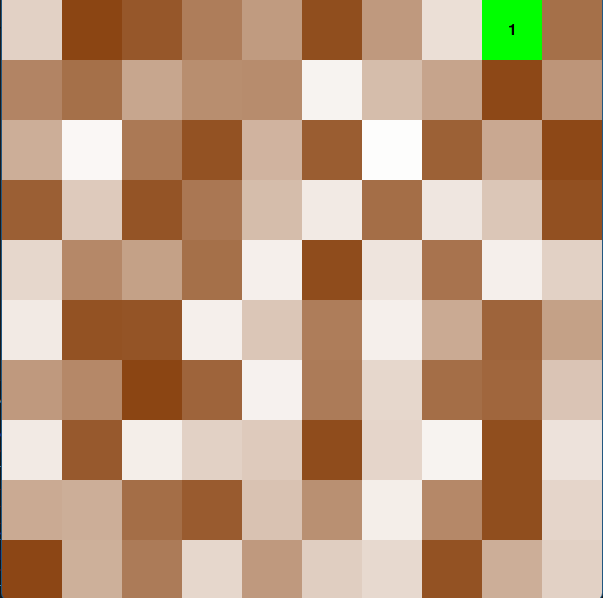
\includegraphics[width=0.18\textwidth]{images/image1.png}\hfill
    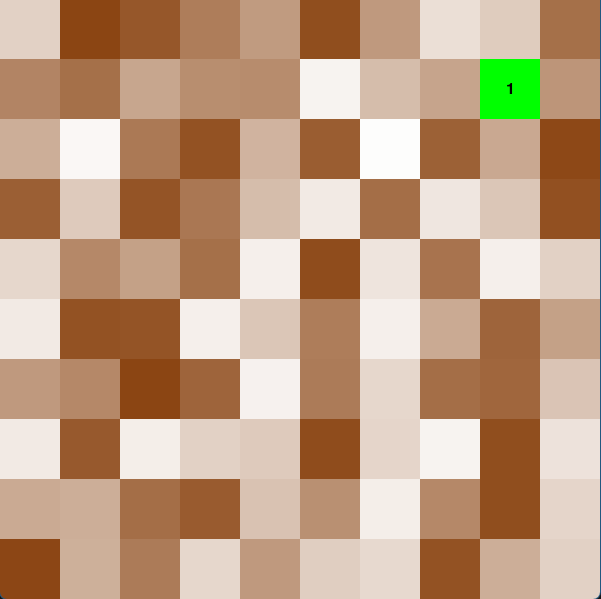
\includegraphics[width=0.18\textwidth]{images/image2.png}\hfill
    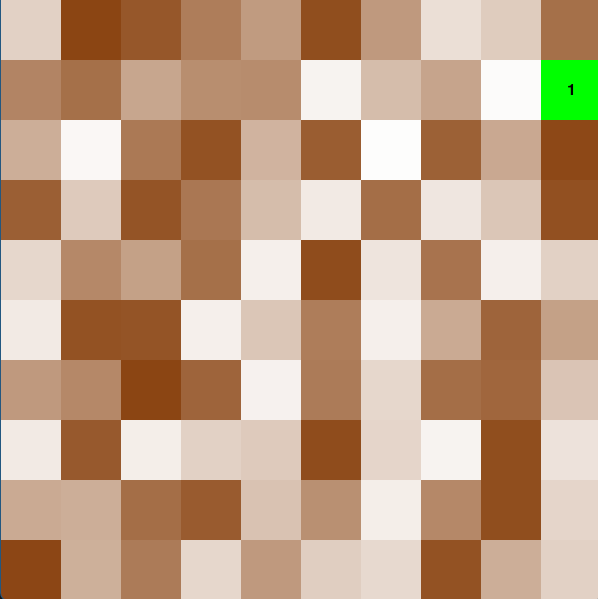
\includegraphics[width=0.18\textwidth]{images/image3.png}\hfill
    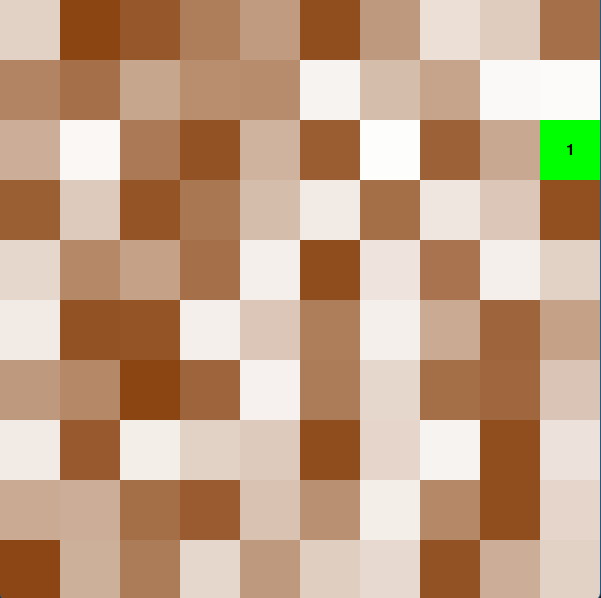
\includegraphics[width=0.18\textwidth]{images/image4.png}
    \caption{Secuencia de movimientos del agente FoodSeekerAgent en la simulación desde la posicion \( (0, 8) \) hasta \( (2, 9) \) .}
\end{figure}

\paragraph{Implementación}
Para implementar el A* en la simulación de nuestro juego, utilizamos una clase que gestiona la verificación de movimientos válidos y obstáculos. Esta clase ajusta el algoritmo para adaptarse a las características específicas del entorno de juego, como áreas inaccesibles y diferentes costos de movimiento asociados con diversos tipos de terreno.

\subsubsection{Búsqueda en Amplitud (BFS)}
La Búsqueda en Amplitud, o BFS por sus siglas en inglés (Breadth-First Search), es un algoritmo clásico para explorar grafos y árboles. Es especialmente útil en situaciones donde necesitamos encontrar el camino más corto en términos de número de aristas entre un nodo de origen y otros nodos, dado que explora todos los nodos a la misma profundidad antes de moverse a la profundidad siguiente.
En nuestra simulación está especialmente diseñado para calcular rutas de escape en situaciones donde un agente necesita maximizar la distancia de un atacante en un entorno de grilla. La adaptación permite a los usuarios elegir entre obtener sólo el siguiente movimiento óptimo o el camino completo de escape.

\paragraph{Funcionamiento de BFS}
La implementación de BFS comienza con la inserción del nodo de origen en una cola. A medida que cada nodo se procesa, sus vecinos no visitados se añaden al final de la cola. Este proceso continúa hasta que se visitan todos los nodos alcanzables o hasta que se encuentra el nodo objetivo, lo que permite una exploración completa en capas.

\begin{itemize}
    \item \textbf{Cola de BFS}: Utilizamos una cola para mantener el orden de exploración de los nodos. En nuestra implementación, esto se maneja con una estructura de datos deque para una eficiente inserción y eliminación de elementos.
    \item \textbf{Conjunto de Obstáculos y Visitados}: Mantenemos un conjunto de obstáculos para evitar la exploración de nodos no transitables y un conjunto de nodos visitados para evitar procesar el mismo nodo más de una vez.
    \item \textbf{Validación de Movimientos}: Cada movimiento potencial se valida para asegurar que no se salga del límite del entorno de juego y no se encuentre con obstáculos.
\end{itemize}

\paragraph{Ejemplo de Uso}
En el siguiente ejemplo, mostramos un agente del tipo $PacifistAgent$ \( (azul) \) en la posicion \( (5, 6) \), que en nuestra simulación representa al agente que tiene una estrategia pacifica, evade los ataques e intenta sobrevivir.
En este caso, tenemos un tablero de \(7 \times 7\). Definimos la posición inicial del agente $CombatantAgent$ \( (rojo) \) como \( (3, 3) \). La salida del algoritmo proporcionará la secuencia de movimientos para llegar a la posición segura más lejana posible, evitando al atacante, evidenciamos en las siguientes imagenes como
la secuencia de movimientos incluye como primer movimiento el de alejarce del atacante hacia la casilla \( (6, 6) \), luego en el siguiente movimiento, este se queda en esa misma posicion ya que de entre las posibles es la mas lejana al atacante


\begin{figure}[H]
    \centering
    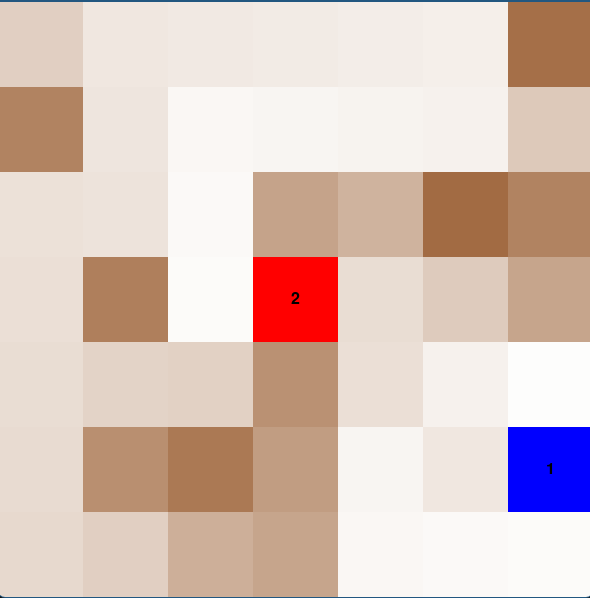
\includegraphics[width=0.18\textwidth]{images/image6.png}\hfill
    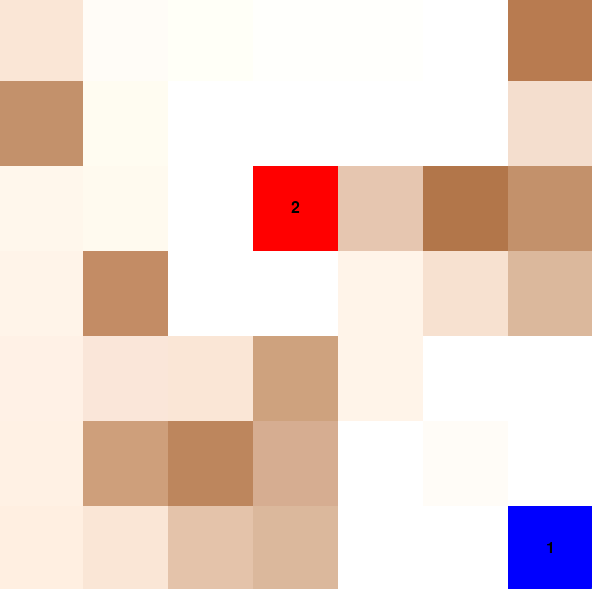
\includegraphics[width=0.18\textwidth]{images/image7.png}\hfill
    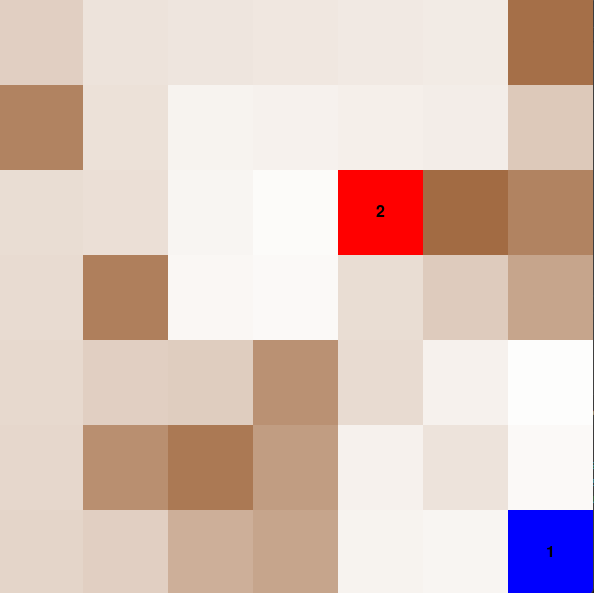
\includegraphics[width=0.18\textwidth]{images/image8.png}
    \caption{Secuencia de movimientos calculada por BFS para evadir al atacante, mostrando cada paso desde el inicio hasta la posición segura más lejana posible.}
\end{figure}

\paragraph{Implementación}
Nuestra clase \textit{BFS} incluye métodos para configurar los obstáculos y calcular la ruta basada en las posiciones dinámicas de los agentes y las barreras en el entorno. Esto asegura que el agente siempre tenga una ruta de escape actualizada y pueda reaccionar a los cambios en el entorno.



\subsubsection{Monte Carlo Tree Search (MCTS) (Trabajo en proceso)}
El Monte Carlo Tree Search (MCTS) es un algoritmo de búsqueda heurística ampliamente utilizado en la toma de decisiones en juegos y problemas de optimización combinatoria.
A diferencia de otros enfoques, como la búsqueda en profundidad, MCTS no requiere un conocimiento completo del espacio de búsqueda y es especialmente útil en entornos con una gran cantidad de acciones posibles y una complejidad elevada.\\

Este método se basa en una búsqueda inteligente de árboles que equilibra la exploración y la explotación. Utiliza el concepto de muestreo aleatorio mediante simulaciones, conocidas como "playouts", para evaluar las diferentes opciones disponibles.
A medida que se realizan más playouts, el algoritmo acumula estadísticas sobre las acciones tomadas.\\

En nuestra implementación, aplicamos MCTS para guiar al agente en la selección de acciones óptimas en un entorno simulado. Consideramos el limitado conocimiento del usuario sobre la simulación para adaptar la exploración del árbol de búsqueda
y priorizar aquellas acciones que parecen más prometedoras según las heurísticas de comportamiento implementadas en los agentes.\\

\paragraph{Funcionamiento de MCTS}
Cada vez que un agente emplea MCTS en la toma de decisiones, se crea un objeto MCTS que representa el árbol de búsqueda del agente en ese turno. La raíz de este árbol refleja el estado de la simulación justo antes de que el agente tome una decisión.
El algoritmo de MCTS sigue un ciclo de cuatro pasos:\\

\begin{itemize}
    \item \textbf{Selección}: Desde el nodo raíz R, se busca un nodo hoja L que represente un escenario de la simulación desde el cual no se ha tomado ninguna decisión.
    \item \textbf{Expansión}: A menos que el nodo L sea terminal (es decir, el agente gana o pierde), se expande el árbol de búsqueda creando uno o más nodos secundarios. Estos nodos representan movimientos válidos desde la posición de juego definida por L.
    \item \textbf{Simulación}: Se realiza una reproducción aleatoria del juego desde el nodo C, elegido durante la fase de expansión. Esta simulación proporciona una estimación del valor de ese nodo y ayuda a evaluar la calidad de las acciones disponibles.
    \item \textbf{Actualización}: El resultado de la simulación se utiliza para actualizar la información en los nodos de la ruta desde C hasta R, lo que permite al algoritmo ajustar sus estimaciones y mejorar la toma de decisiones futuras.
\end{itemize}

\paragraph{Implementación}
En nuestra implementación de MCTS, aprovechamos la información observada por el agente y su conocimiento previo de la simulación, como los agentes que ha visto cercanos o el recuento global de muertes, para construir una representación simplificada del escenario.

\paragraph{Ejemplos}
Ejemplos...



\subsection{LLM}
Utilizamos el LLM para la creación de agentes y la configuración del escenario de la simulación, así como para la función de comentarista del juego. Para la creación de agentes, empleamos una lista con descripciones por defecto de los comportamientos de nuestros tipos de personajes y la información suministrada por el usuario. El LLM infiere cuál es el tipo de personaje por defecto que más se acerca a la descripción del usuario, así como las estadísticas, teniendo en cuenta la mención u omisión de aspectos positivos y negativos en la descripción del personaje.
\\
En cuanto a la creación del mapa, se eligen las dimensiones del escenario a simular de acuerdo a la inferencia realizada por el LLM en la descripción del terreno.  \\
Para la función de comentarista, alimentamos al LLM con las últimas acciones ocurridas en la simulación y las descripciones de los personajes. Esto permite al modelo crear un breve relato de los eventos más recientes no comentados en la simulación.
\subsection{Interfaz de la simulación}

\section{Análisis de la simulación}
\section{Conclusiones}

\end{document}
